% !TEX encoding = UTF-8
% !TEX TS-program = pdflatex
% !TEX root = ../tesi.tex

%**************************************************************
\chapter{Verifica e validazione}
\label{cap:verifica-validazione}
%**************************************************************
\intro{In questo capitolo viene approfondito il periodo di verifica e test, durante il quale sono emerse alcune difficoltà che hanno richiesto un tempo maggiore del previsto per la risoluzione. Viene qui presentata la modalità di risoluzione di queste difficoltà, unita ai risultati ottenuti durante i test e i dati emersi dalle analisi dei risultati.}
%**************************************************************
\section{Generazione degli input}
Una volta accertatami che il comportamento della \emph{\gls{bus-logic}}\glsfirstoccur\ del software prodotto fosse corretto su piccoli input di prova, si è presentato il problema di testare l'applicazione su istanze di input più grandi e con più variabili. Da piano di lavoro, il tempo previsto per verifica, testing e analisi dei risultati era stabilito di 20 ore; tuttavia, è stato da subito chiaro che il processo di verifica sarebbe stato più complicato del previsto.\\
Per eseguire test significativi in serie, era infatti necessario poter produrre automaticamente degli input su cui il software potesse elaborare per produrre scheduling: è stata quindi estesa la classe \texttt{Excel} per poter andare a modificare in scrittura i fogli xls di input. In un primo momento, si è provato a generare degli input randomici, ma tale soluzione si è rivelata problematica per due motivi: in primo luogo, gli input randomici non producevano praticamente mai delle soluzioni ammissibili in quanto spesso ci si trovava con un sbilanciamento postazioni/lavoratori; in secondo luogo, anche quando veniva (raramente) prodotta una soluzione ammissibile, tale soluzione non poteva essere rappresentativa di un buono scheduling in quanto non era sensata. Il problema principale da risolvere è quindi diventato \textit{come} generare degli input il più possibile vicini alla realtà che potessero produrre degli scheduling da analizzare.\\
Il problema è stato esposto al tutor aziendale, che ha approvato la modifica al piano di lavoro assegnando più ore alla verifica e al testing, tagliando su attività per il raggiungimento di requisiti desiderabili e opzionali, ritenendo più importante poter testare il software in maniera corretta e approfondita. \\
\\
Secondo le informazioni fornite dal casinò, gli input per essere realistici dovevano:
\begin{itemize}
    \item comprendere circa 30 postazioni aperte contemporaneamente, per un totale di 40 lavoratori attivi. Il totale dei lavori, per garantire quindi uno scheduling fair e rispettoso delle pause e dei vincoli previsti, doveva ammontare a circa il 33\%\ in più rispetto al numero di postazioni.
    \item di tutte le postazioni aperte, alla maggior parte viene assegnato un livello basso e giochi comunemente conosciuti dai lavoratori, mentre le postazioni che richiedono un livello alto o giochi poco conosciuti sono meno.
    \item il livello dei lavoratori dipende dal tempo passato all'interno del casinò e dalle loro abilità, di conseguenze la maggior parte dei lavoratori è di livello intermedio, mentre sono pochi quelli di livello molto alto e molto basso.
    \item i giochi conosciuti dai lavoratori dipende dal loro livello: più un dealer è di livello alto, più giochi conosce; per quanto riguarda inspector e dealer-inspector, essi conoscono praticamente tutti i giochi.
\end{itemize}
Sulle basi di queste informazioni, è stato possibile produrre un modello probabilistico che descrivesse una situazione reale e progettare una nuova classe, \texttt{Test}, che generasse automaticamente ad ogni \textit{run} dell'algoritmo un set di input secondo il modello definito.

\subsection{Modello probabilistico}

Tutti i grafici presenti in questa sezione sono stati prodotti sul sito di Wolfram Alpha\footcite{https://www.wolframalpha.com/examples/StatisticalDistributions.html}.
    \paragraph{Numero di postazioni} Ipotizzando che il numero di postazioni aperte contemporaneamente sia circa 30, genero il numero di postazioni tramite una distribuzione normale $\mathcal{N}(\mu;\sigma \ap{2})$ con:
    \begin{itemize}
        \item tavoli: $\mu = 20$, $\sigma \ap{2} = \frac{\mu}{5}$
        \item pit: $\frac{tavoli}{3}$
    \end{itemize}

    \begin{figure}[!htb]
    \begin{widepage}
    \centering
    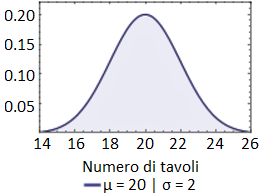
\includegraphics[width=.49\textwidth]{../immagini/gauss_tavoli_w.png}\hfil
    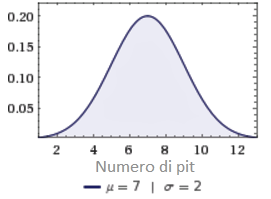
\includegraphics[width=.49\textwidth]{../immagini/gauss_pit_w.png}
    \caption{Distribuzioni normali per il numero di postazioni}
    \end{widepage}
    \end{figure}
\clearpage
    \paragraph{Costruzione delle postazioni} Ipotizzando che le postazioni che richiedono un livello alto sono poche e viceversa, genero i livelli delle postazioni L\ped{t} con una distribuzione discreta uniforme $\mathcal{U}(\mathcal{S})$ dove \[\mathcal{S} = \{ \alpha + i*\beta \text{ t.c. } i \in \{0,2,...,n\} \} \] ovvero i cui elementi sono i progressione aritmetica con $\alpha = 1$, $\beta = 1$ e:
    \begin{itemize}
        \item per i tavoli (8 livelli): $n = 7$
        \item per i pit (3 livelli): $n = 2$
    \end{itemize}
    \begin{figure}[!htb]
        \begin{widepage}
            \centering
            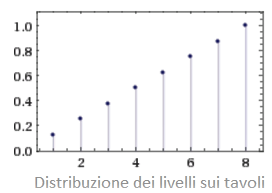
\includegraphics[width=.49\textwidth]{../immagini/discr_livelli_tavoli.png}\hfil
            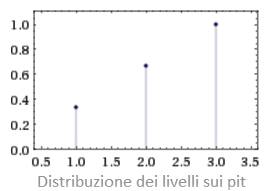
\includegraphics[width=.49\textwidth]{../immagini/discr_livelli_pit.png}
            \caption{Distribuzione discreta uniforme per i livelli delle postazioni}
        \end{widepage}
    \end{figure}
    \FloatBarrier
    \noindent
    Inoltre viene generato il gioco richiesto ad una certa postazione in modo che la frequenza del gioco base (//) sia doppia rispetto a quella di altri giochi (BJ e PG).\\
    Ad ogni postazione è richiesto un solo gioco.
    
    \begin{figure}[!htb]
        \begin{widepage}
            \centering
            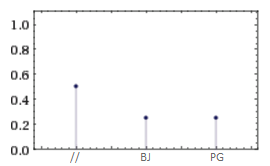
\includegraphics[width=.49\textwidth]{../immagini/distr_giochi_tavoli.png}
            \caption{Frequenza di estrazione dei giochi per ogni postazione}
        \end{widepage}
    \end{figure}%
    \clearpage
    \paragraph{Numero di lavoratori} Ipotizzando che il numero di lavoratori attivi contemporaneamente sia di circa il 33\% in più rispetto al numero di postazioni, genero il numero di lavoratori tramite una distribuzione normale $\mathcal{N}(\mu;\sigma \ap{2})$ con:
    \begin{itemize}
        \item dealer: $\mu = tavoli*1.6$, $\sigma \ap{2} = \frac{tavoli}{5}$
        \item inspector: $\mu = pit*1.6$, $\sigma \ap{2} = \frac{pit}{5}$
    \end{itemize}

    \begin{figure}[!htb]
        \begin{widepage}
        \centering
        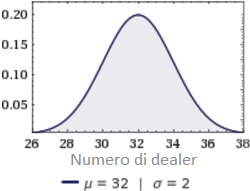
\includegraphics[width=.49\textwidth]{../immagini/gauss_dealer_w.png}\hfil
        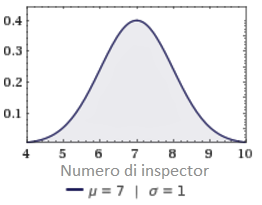
\includegraphics[width=.49\textwidth]{../immagini/gauss_inspector_w.png}
        \caption{Distribuzioni normali per il numero di lavoratori}
        \end{widepage}
    \end{figure}
    \FloatBarrier
    \noindent
    Da notare che il valor medio $\mu$ è stato fissato al 60\% in più rispetto al numero di postazioni, sarà poi compito dell'algoritmo andare ad ottimizzare il numero di lavoratori richiesti per riempire lo scheduling. \\
    \\
    Per quanto riguarda il numero di dealer-inspector, esso viene fissato a \[(tavoli + pit) * 1.6 - dealer - inspector\] per far sì che il numero di lavoratori attivi sia sempre esattamente il 60\% in più rispetto al numero di postazioni.
    \clearpage
    \paragraph{Costruzione dei lavoratori} Ipotizzando che il livello dei lavoratori dipenda solo dal tempo che hanno passato all'interno del casinò, generiamo i livelli dei lavoratori L\ped{w} tramite una distribuzione normale $\mathcal{N}(\mu;\sigma \ap{2})$ con:
    \begin{itemize}
        \item dealer: $\mu = 4.5$, $\sigma \ap{2} = \frac{\mu}{3.5}$
        \item inspector: $\mu = 2$, $\sigma \ap{2} = \frac{\mu}{1}$
    \end{itemize}
     \begin{figure}[!htb]
         \begin{widepage}
             \centering
             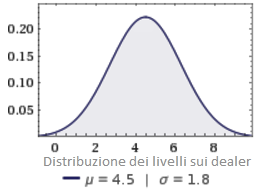
\includegraphics[width=.49\textwidth]{../immagini/livelli_dealer.png}\hfil
             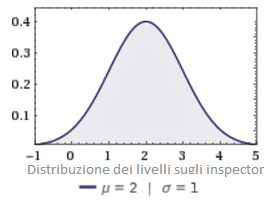
\includegraphics[width=.49\textwidth]{../immagini/livelli_insp.png}
             \caption{Distribuzioni normali per i livelli dei lavoratori di lavoratori}
         \end{widepage}
     \end{figure}
     \FloatBarrier
     \noindent
     Ipotizzando che la probabilità che un lavoratore conosca un gioco sia direttamente proporzionale al suo livello (più un lavoratore ha livello alto, più giochi conosce; tutti conoscono i giochi base //), generiamo i giochi che ogni lavoratore conosce con una distribuzione di Bernoulli $\mathcal{B}e(p)$ dove $p = 1 - \frac{livello}{10}$.
     \begin{figure}[!htb]
         \begin{widepage}
             \centering
             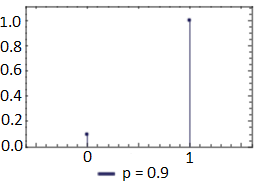
\includegraphics[width=.49\textwidth]{../immagini/livello_1.png}\hfil
             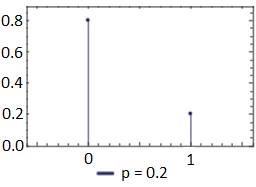
\includegraphics[width=.49\textwidth]{../immagini/livello_8.png}
             \caption{Probabilità che due lavoratori di livelli 1 (a sinistra) e 8 (a destra) conoscano un gioco (1) o meno (0)}
         \end{widepage}
     \end{figure}
 \clearpage
\subsection{Progettazione}
%**************************************************************
\section{Esiti dei test}